\section{Arquitectura del sistema}
	\label{sec:interlockingArch}
	
	Cada módulo del sistema fue implementado con máquinas de estado finitas	con camino de datos (FSMD, del inglés Finite State Machine with Data path), que son máquinas de estado finitas (FSM, del inglés Finite State Machine) y circuitos
	secuenciales y combinacionales que constituyen el camino de datos. Utilizar una FSMD aporta un mayor control del diseño a bajo nivel, una mayor portabilidad y un mas eficiente uso de los recursos de la plataforma electrónica.
	
	Una FSMD, cómo la ilustrada en la Figura \ref{fig:FSMD}, posee dos partes diferenciadas: el camino de control y el camino de datos. El camino de control se compone de una FSM que, según las entradas de control y el estado interno que posee, genera señales internas que controlan los circuitos secuenciales del camino de datos. Estos, a su vez, contienen los bloques que procesan las entradas y actúan sobre las salidas.
	
	\begin{figure}[H]
		\centering
		\includegraphics[width=1\textwidth]{Figuras/FSMD.png}
		\centering\caption{Diagrama en bloques  de una FSMD genérica.}
		\label{fig:FSMD}
	\end{figure}
	
	El ACG generará automáticamente cada FSMD en función de los elementos detectados en la red de grafos. Es decir, el modelado de cada elemento será una plantilla que contemplará todos los casos posibles, con todas las entradas y salidas posibles, pero solo se implementarán las funcionalidades que cada elemento particular requieran. De esta manera, será posible optimizar los recursos a la vez que se valida cada elemento una única vez, como un objeto genérico.
	
	Los elementos ferroviarios a ser modelados por el ACG son los que denominaremos elementos dinámicos. Es decir, todo elemento ferroviario que posea algún estado susceptible de modificarse en función de algún evento o del tiempo. Estos elementos dinámicos pueden adoptar los siguientes estados:
	
	\begin{itemize}
		\item Circuitos de vía: ocupados, desocupados.
		\item Rutas: no solicitadas, solicitadas.
		\item Señales: rojo, doble amarillo, amarillo, verde
		\item Pasos a nivel: barrera baja, barrera alta.
		\item Cambios de vías simples: posición normal, posición reversa.
		\item Cambios de vías dobles: posición doble normal, posición doble reversa, posición normal reversa, posición reversa normal.
		\item Cambios de vias en tijeras: posición normal, posición reversa.
	\end{itemize}
	
	Internamente, el sistema contemplará que algunos elementos pueden admitir estados de transición. Estos estados son producto del tiempo que requiere un actuador para completar las comandos que la FPGA envía. No obstante, los estados de transición solo serán tolerados un tiempo determinado, pasado el cuál se asumirá que la orden no fue completada y se abortará la ejecución de la ruta solicitada.
	
	La arquitectura general del sistema generado por el ACG se ilustra en la Figura \ref{fig:GeneralSystem}. El módulo \textit{Detector} recibe las tramas en formato serie, comprueba su integridad y en caso de que los datos contengan solamente caracteres válidos los entrega al módulo \textit{Decoder}. El módulo \textit{Decoder} toma esos datos y los paraleliza para entregarlos al módulo \textit{Network} en la entrada que corresponda a cada dato. El módulo \textit{Network} es la implementación de la red de grafos generada por el RNA. 
	
	\begin{figure}[H]
		\centering
		\includegraphics[width=1\textwidth]{Figuras/Arq_general.png}
		\centering\caption{Arquitectura general del sistema generado por el ACG.}
		\label{fig:GeneralSystem}
	\end{figure}
	
	El módulo \textit{Encoder} toma las salidas generadas por el módulo \textit{Network}, las agrupa apropiadamente y se las suministra al módulo] \textit{Printer}. El módulo \textit{Printer} transforma cada elemento de la señal en un caracter imprimible para enviar a la UART. Finalmente, el módulo \textit{Selector} se usa exclusivamente a los fines de comprobar el correcto funcionamiento de la comunicación serie, puenteando a todos los otros módulos.
	
	La descripción del sistema se realizará desde sus módulos mas externos, que implementan la comunicación del sistema: los módulos de UART, Detector, Decoder, Encoder y Printer. De forma tal de entender en alto nivel como es el proceso de comunicación hacia y desde la FPGA, para luego abordar el núcleo del sistema de enclavamiento. cuya complejidad es mucho mayor.		
	
	\subsection{Modulo UART}
\label{sec:UART}
	Si consideramos la lista de elementos dinámicos y cada estado que pueden admitir, es claro que la cantidad de señales sobrepasaría por mucho la limitada cantidad de puertos que una FPGA pueda proveer. Por ejemplo, si se considera un sistema ferroviario como el presentado en la Figura \ref{fig:bypass_1}, que por comodidad para el lector se copia en la Figura \ref{fig:bypass_3}, seria necesario mas de 25 pines de la FPGA entre entradas y salidas, lo que implicaría que para ese sistema tan simple se requeriría utilizar una FPGA de tamaño medio o grande. Esto implica que ese enfoque dificultaría la implementación del sistema de enclavamiento de redes ferroviarias de mayor tamaño.
	
	\begin{figure}[H]
		\centering
		\includegraphics[width=1\textwidth]{Figuras/bypass}
		\centering\caption{Topología de derivación ferroviaria.}
		\label{fig:bypass_3}
	\end{figure}
	
	Es por eso que se decidió que la FPGA mediante la cual se implemente el sistema de enclavamiento debe recibir y transmitir la información a la cabina de señalamiento en formato serie. El uso de comunicación serie para la implementación del sistema es apropiado, ya que otros sistemas ferroviarios utilizan comunicación serie, como por ejemplo RS-485 o MVB en las redes de comunicación de trenes (TCN, del inglés \textit{Train Communication Network}) \cite{TCN}. La comunicación a implementar entre el sistema de enclavamiento y la cabina de señalamiento deberá ser flexible para ser utilizada en diferentes implementaciones con menor o mayor cantidad de elementos ferroviarios.
	
	En la Figura \ref{fig:GeneralCom} se presenta la propuesta de conexión de la FPGA con una computadora externa, que para el desarrollo y prueba de la solución hará las veces de la cabina de señalamiento. En la Figura \ref{fig:GeneralCom} también se representan los módulos internos de comunicación. La UART (del inglés \textit{Universal Asynchronous Receiver-Transmitter}), junto con las memorias FIFO (del inglés \textit{First-In First-Out}), se utilizan para implementar el intercambio de las tramas de datos entre la FPGA y la computadora.
	
	\begin{figure}[H]
		\centering
		\includegraphics[width=0.7\textwidth]{Figuras/UART_module.png}
		\centering\caption{Conexión entre la FPGA y una computadora externa.}
		\label{fig:GeneralCom}
	\end{figure}
	
	El módulo de recepción (UART RX), que se ilustra en la Figura \ref{fig:GeneralCom}, es el encargado de procesar cada bit recibido con un baudrate preestablecido y almacenar cada bit en la FIFO RX. Al completarse un byte de datos, será enviado al sistema de enclavamientos, junto con una serie de pulsos para indicar cuándo deben ser leídos. El sistema de enclavamientos esperará a tener la cantidad de bytes necesarios (definidos por el ACG) para empezar a procesar la trama. Luego, el sistema de enclavamientos devolverá una nueva trama de bytes a la FIFO TX. Finalmente la nueva trama será enviada al módulo de transmisión (UART TX) que enviará la información bit a bit, con el mismo baudrate que fue recibido.
		
	En la Figura \ref{fig:Stream} se ilustra el formato definido para las tramas de entrada y salida. La trama tendrá un tamaño de entrada N y de salida M, con N igual que M. La cantidad de cada elemento ferroviario es definida por el RNA y el orden de los elementos es fijo y definido en el ACG. Los elementos que no existan en la locación analizada tendrán paquetes de datos de largo nulo. Además, la trama tendrá un caracter delimitador de entrada y de salida ($<$ y $>$ respectivamente). Todos los elementos de la trama serán hexadecimales en formato ASCII, para poder ser interpretados fácilmente en una terminal y ser menos susceptibles a errores por alteraciones en algún bit aleatorio.
	
	\begin{figure}[H]
		\centering
		\includegraphics[width=1\textwidth]{Figuras/Tramas.png}
		\centering\caption{Tramas de datos y paquete de datos.}
		\label{fig:Stream}
	\end{figure}
	
	El largo de la trama de entrada y de salida queda definido por la Ecuación \ref{eq:StreamLength_in}. 
	
	\begin{equation} 
		\label{eq:StreamLength_in}
		\text{N} = 1\text{byte} (\text{N}_{NET}+\text{N}_{\text{RTS}}+\text{N}_{\text{LCB}}+\text{N}_{\text{SSW}}+\text{N}_{\text{SCR}}\text{N}_{\text{SIG}}+\text{N}_{\text{DSW}})
	\end{equation}
	
	Cada elemento dinámico requiere un sólo caractér hexadecimal para definir su estado utilizando sus 4 bits. Los 2 bits menos significativos definen el estado (\textit{STATE} en Figura \ref{fig:Stream}). Por ejemplo, la posición de un cambio de vías o el aspecto de una señal. Los 2 bits mas significativos definen el enclavamiento del elemento dinámico (\textit{LOCK} en la Figura \ref{fig:Stream}). El parámetro \textit{Lock} puede tomar tres valores: '00' para elementos disponibles, '01' para elementos que han sido reservados por una ruta pero aún no han sido enclavados y '10' para elementos enclavados.
	
	En la Figura \ref{fig:Stream_ejemplo1} se ilustran dos tramas recibidas en el caso de una topología ferroviaria que será explicada en profundidad en la Sección \ref{sec:ejemplo_1}.  La primer trama de datos representada el estado del sistema de enclavamiento cuando no se han solicitado rutas y la segunda ilustra una ruta pedida y habilitada. Ambas tramas cuentan con 11 netElements, 21 rutas, 23 señales, 2 pasos a nivel, 5 cambios de vías y los correspondientes tags iniciales y finales.
	
	En la primer trama se pueden apreciar: 11 secciones de vías sin ocupar (todos los valores en 1), 21 rutas sin solicitar (todos los valores en 0), 23 señales de las cuales podemos destacar 14 señales rojas (valores en 0), 4 señales naranjas (valores en 1), 3 señales amarillas (valores en 2) y 2 señales verdes (valores en 3). Además, la trama describe dos pasos a nivel con el brazo de barrera en alto (todos los valores en 1) y 5 cambios de vías, 3 de ellos en posición normal (valores en 0) y 2 en posición reversa (valores en 1). Debido que no existen rutas solicitadas ni habilitadas en esta trama (todos los valores en 0), todos los elementos tienen sus valores de LOCK en '00', lo que indica que se encuentran disponibles para ser enclavados por la ruta correspondiente.
	
	\begin{figure}[H]
		\centering
		\includegraphics[width=1\textwidth]{Figuras/Trama_ejemplo.png}
		\centering\caption{Tramas de datos y paquete de datos.}
		\label{fig:Stream_ejemplo1}
	\end{figure}

	En la segunda trama, en cambio, se puede apreciar que el primer netElement (ne1) es representado con un 8 (1000), lo cual significa que se encuentra enclavado (10) y ocupado (00). Los netElements ne9 y ne15 son representados con un 9 (1001), ya que también se encuentran enclavados (10), pero no han sido ocupados (01). Además, la ruta 12 es representada con un 7 (0111), el estado de liberación secuencial (que será explicado en la Sección \ref{sec:ACG_rts}). Los semáforos que presentan valores superiores a 4 (0100) son aquellos que se encuentran reservados y los que presentan valores superiores a 8 (1000) se encuentran enclavados. En este caso, el semáforo S22 se representa con un 7 (0111, verde y reservado) y el semáforo T05 se representa con un 8 (1000, rojo y enclavado). Finalmente, los cambios de vías pares se encuentran en posición normal y los impares en posición reversa. En el caso del cambio de vías sw04, el valor 9 representa un cambio de vías enclavado en posición reversa y el cambio de vías sw07, el valor 8 representa un cambio de vías enclavado en posición normal.
	
	La implementación de los módulos de transmisión y recepción de la UART es invariante para cada locación, es decir, los recursos asignados serán los mismos, cualquiera sea el tamaño del sistema a implementar. Los módulos de memorias FIFO, en cambio, dependen de las características y del tamaño del sistema. Locaciones mas complejas tendrán valores de N y M mayores y, por lo tanto, requerirán FIFOs mas grandes. 
	
	
	
	
	%11111111111000000000000000000000101203210000000000120301110010
    %81191119111000000000000700000000171203210000000810120301190080
	
	
	%Con este criterio de diseño, en todos los demás casos, la FIFO de salida tendrá el mismo tamaño que la FIFO de entrada o a lo sumo será 50 \% menor, lo que representa un ahorro de 25 \% de los recursos estimados. Por ejemplo, si se necesita que la entrada tenga 15 bits y la salida 7 bits y se le asignara el mismo tamaño a ambas FIFOs; tanto la FIFO de entrada como la de salida necesitarán 16 bits cada una, dando un total de 32 bits. Pero si se aplica el criterio de tamaños desacoplados, entonces para la FIFO de salida podrían asignarse solamente 8 bits, dando un total de 24 bits, un 25 \% menos que los 32 bits que necesitaría si ambas FIFOs quedaran definidas según los datos de la entrada.
	\subsubsection{Módulo Detector}

\lipsum[1]

El módulo detector tiene como función recibir una secuencia de caracteres y armar una salida con un vector de elementos booleanos. Un diagrama en bloques del funcionamiento del módulo se muestra en la figura 3.9

\begin{figure}[H]
	\centering
	\includegraphics[width=1\textwidth]{example-image}
	\centering\caption{FPGA.}
	\label{fig:XXX}
\end{figure}

La UART envía secuencialmente un caracter por medio de la señal r\_data (8 bytes) y un pulso (r\_disponible) para informar que un nuevo dato ha sido enviado, además de indicar por medio de la señal N la cantidad de caracteres que serán
enviados.

El proceso de detección se ilustra en la figura 3.10.

\begin{figure}[H]
	\centering
	\includegraphics[width=1\textwidth]{example-image}
	\centering\caption{FPGA.}
	\label{fig:XXX}
\end{figure}

En la figura 3.10 se tiene un estado inicial en el cual se espera el caracter de inicio de la trama ("<") que provoca una transición al estado de lectura. En dicho estado se recibirán hasta N caracteres mientras se actualiza un contador interno. Cuando el contador interno iguale la cantidad N, se verifica si el próximo caracter es el de
fin de trama (">"). 

Si el caracter leído es el de final de trama, se pasa al estado final, donde el paquete es considerado válido y enviado a la próxima etapa junto con su pulso de validación del dato. Si el caracter leído es distinto, entonces se descarta toda la trama y se vuelve al inicio a la espera de otro caracter de inicio de trama, reiniciando
todas las variables auxiliares.

Internamente se tienen diversas variables auxiliares para controlar si se han recibido los delimitadores y si la cantidad recibida es correcta. Eso cobra gran importancia al realizar los ensayos, porque se puede diferenciar rápidamente la fuente de posibles errores.
	\subsection{Módulo Decoder}

El módulo \textit{Decoder} es el encargado de demultiplexar la trama \textit{packet}[N] ya validada por el módulo \textit{Detector}. El módulo \textit{Decoder} recibe el vector de elementos booleanos \textit{packet}[N] y la señal \textit{process} que indica cuando puede iniciar el proceso de demultiplexación. La salida serán todos los vectores de estado de los elementos ferroviarios, si existen. El diagrama de bloques de las máquinas de estado finitas con camino de datos se muestra en la Figura \ref{fig:Decoder_module}.

\begin{figure}[H]
	\centering
	\includegraphics[width=1\textwidth]{Figuras/Decoder_module.png}
	\centering\caption{FSMD del módulo \textit{Decoder}.}
	\label{fig:Decoder_module}
\end{figure}

Esta demultiplexación no es ni equitativa para todos los vectores de salida, ni tampoco existirán todos los vectores de salida. La porción de \textit{packet}[N] correspondiente a cada vector será en función de la cantidad de elementos de cada tipo presentes en la locación. Esto ya fue calculado previamente por el ACG y explicado en la Sección \ref{sec:UART} al definir el formato de la trama. Si la cantidad de un cierto elemento ferroviario es mayor que uno, el ACG implementará el estado de ese elemento con un \textit{std\_logic\_vector} del tamaño adecuado. Si solo existe un elemento ferroviario de ese tipo, el ACG implementará un \textit{std\_logic}. Si no existiese ningún elemento ferroviario en la locación, el ACG no implementará ninguna de las funcionalidades relativas a dicho elemento, optimizando el uso de recursos en la FPGA.
	\subsubsection{Módulo Encoder}

\lipsum[1]
	\subsection{Módulo Printer}
	\label{sec:printer}
	
	El módulo Printer (ver Figura \ref{fig:GeneralSystem}) realiza la conversión de cada elemento de un vector de M elementos hexadecimales (\textit{packet}[M], M elementos de 4 bits) en caracteres hexadecimales (1 byte). Cada elemento del vector es analizado en cada ciclo de reloj (clk\_i) y demultiplexado, de manera tal de convertir un elemento por vez, para luego enviar el byte correspondiente al módulo UART para su posterior transmisión al exterior. El diagrama de bloques de la máquina de estados finitos con camino de datos se muestra en la Figura \ref{fig:Printer_module}.
	
	\begin{figure}[H]
		\centering
		\includegraphics[width=1\textwidth]{Figuras/Printer_module.png}
		\centering\caption{FSMD del módulo \textit{Printer}.}
		\label{fig:Printer_module}
	\end{figure}
	
	En cada ciclo de reloj el módulo \textit{Printer} demultiplexa el vector \textit{packet}[M] para obtener un elemento lógico que procesar, según el valor del contador vigente, que se incrementa en cada ciclo, hasta un máximo de M-1. Si el elemento \textit{packet}[i] es un valor hexadecimal, se enviará un byte equivalente en ASCII. Por ejemplo, se enviará un byte equivalente al 'A' ASCII si el elemento \textit{packet}[i] es una 'A' hexadecimal.
	
	Cada dos ciclos de reloj el módulo \textit{Printer} genera un pulso para habilitar el envío del último byte generado. Junto con el caracter se envía la señal \textit{wr\_uart} para indicarle a la UART que ese dato debe ser guardado en la FIFO de salida y la señal \textit{processed} para indicarle al módulo \textit{Detector} que se pueden procesar nuevas tramas. El ciclo de procesamiento de la trama a transmitir se describe el diagrama de estados de la Figura \ref{fig:Printer_FSMD}.
	
	\begin{figure}[H]
		\centering
		\includegraphics[width=0.8\textwidth]{Figuras/Printer_FSMD.png}
		\centering\caption{Diagrama de estados del módulo \textit{Printer}.}
		\label{fig:Printer_FSMD}
	\end{figure}
	
	El módulo \textit{Printer} inicia por detecto en el estado \textit{restart}, a la espera de recibir la señal \textit{process} del módulo \textit{Encoder}. Se tienen dos estados (\textit{cycle\_1} y \textit{cycle\_2}) para generar el pulso de reloj necesario para mantener sincronizadas las tramas. Cuando el contador haya recorrido los M elementos de \textit{packet}[M], el módulo vuelve al estado \textit{restart}, para esperar una nueva señal \textit{process} para volver a procesar una nueva trama de datos.
	
	Si la trama recibida es incorrecta, o si ya fue impresa, entonces la señal \textit{process} será '0' y el modulo \textit{Printer} dejará de enviar datos a la UART. Si la señal \textit{process} mantiene un estado lógico positivo, el proceso de impresión continuará hasta que la UART indique que no pueda recibir mas datos o que alguna etapa previa informe de algún error en el proceso.
	\subsection{Módulo Selector}
	\label{sec:selector}
	
	Se añadió el módulo \textit{Selector} (ver Figura \ref{fig:GeneralSystem}) para poder facilitar el testeo de la comunicación serial al permitir anular la totalidad del sistema de enclavamiento. De esta manera, es posible validar la lectura, detección y escritura de tramas en bucle en forma independiente al sistema de enclavamiento. Esta funcionalidad es habilitada cambiando la posición de un switch físico de la FPGA y se desactiva invirtiendo su posición. El diagrama de bloques de la máquina de estados finitos con camino de datos diseñado para lograr este objectivo se muestra en la Figura \ref{fig:Selector_module}.
	
	\begin{figure}[H]
		\centering
		\includegraphics[width=0.55\textwidth]{Figuras/Selector_module.png}
		\centering\caption{FSMD del módulo \textit{Selector}.}
		\label{fig:Selector_module}
	\end{figure}
	\subsection{Modulo Network}

\lipsum[1]

\begin{figure}[H]
	\centering
	\includegraphics[width=1\textwidth]{example-image}
	\centering\caption{xxxxx}
	\label{fig:XXXX}
\end{figure}

\lipsum[1]

\subsection{Módulo genérico de las barreras ferroviarias}

\lipsum[1]

\begin{figure}[H]
	\centering
	\includegraphics[width=1\textwidth]{Figuras/LCB_module}
	\centering\caption{FSMD del módulo genérico de \textit{LevelCrossing}.}
	\label{fig:LCB_module}
\end{figure}

\lipsum[1]

\begin{figure}[H]
	\centering
	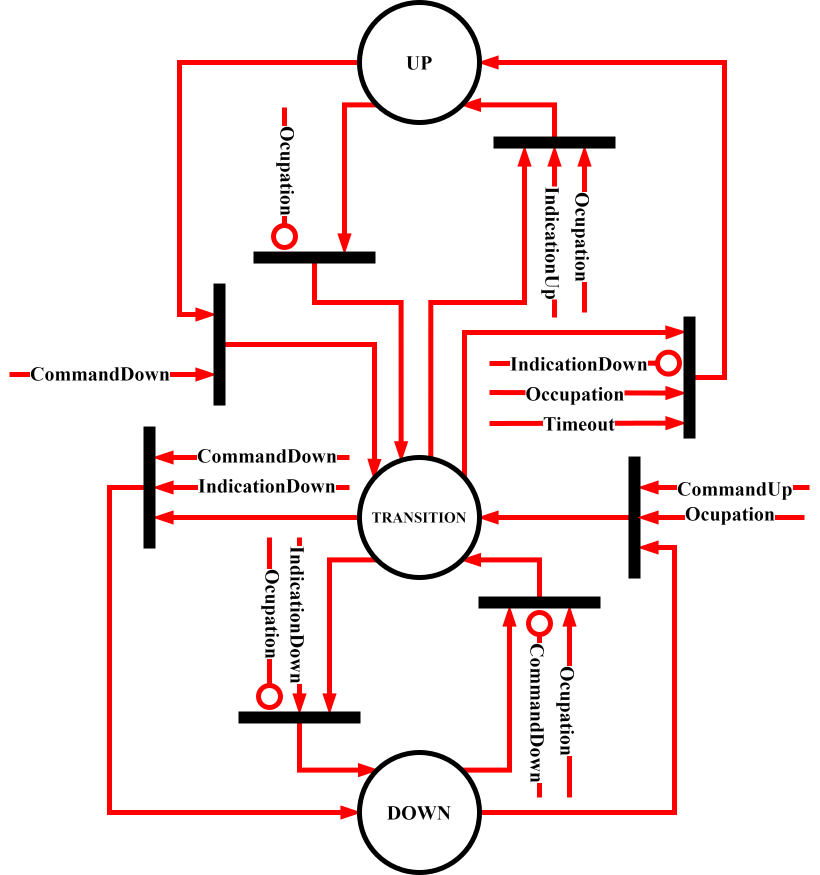
\includegraphics[width=1\textwidth]{Figuras/LCB_petri}
	\centering\caption{Red de petri del modelo dinámico de \textit{LevelCrossing}.}
	\label{fig:LCB_module}
\end{figure}

\lipsum[1]
\subsection{Módulo genérico de los cambios de vías simples}

\lipsum[1]

\begin{figure}[H]
	\centering
	\includegraphics[width=1\textwidth]{Figuras/SSW_module}
	\centering\caption{FSMD del módulo genérico de \textit{SingleSwitches}.}
	\label{fig:SSW_module}
\end{figure}

\lipsum[1]

\begin{figure}[H]
	\centering
	\includegraphics[width=1\textwidth]{Figuras/SSW_Petri}
	\centering\caption{Red de Petri del modelo dinámico de \textit{SingleSwitches}.}
	\label{fig:SSW_Petri}
\end{figure}

\lipsum[1]

\subsection{Módulo genérico de los cambios de vías dobles}

\lipsum[1]

\begin{figure}[H]
	\centering
	\includegraphics[width=1\textwidth]{Figuras/DSW_module}
	\centering\caption{FSMD del módulo genérico de \textit{DoubleSwitches}.}
	\label{fig:DSW_module}
\end{figure}

\lipsum[1]
\subsection{Módulo genérico de los cambios en tijeras}
	\label{sec:ACG_scr}
		
	El módulo \textit{ScissorCrossings} es el encargado de implementar el funcionamiento de los cambios de vías en tijeras en la red ferroviaria. Su implementación es similar a la del módulo \textit{SingleSwitches}, con el ACG utilizando la información otorgada por el RNA para implementar las entradas y salidas necesarias para habilitar el movimiento del cambio de vías solo en situaciones seguras y confirmando su correspondencia mediante la comparación del comando y la indicación. El diagrama de bloques de las máquinas de estado finitas con camino de datos diseñado para lograr este objetivo se muestra en la Figura \ref{fig:SCR_module}.
	
	\begin{figure}[H]
		\centering
		\includegraphics[width=1\textwidth]{Figuras/SCR_module}
		\centering\caption{FSMD del módulo genérico de \textit{ScissorCrossings}.}
		\label{fig:SCR_module}
	\end{figure}
	
	Tal se explicó en la Sección \textit{SingleSwitches}, los cambios de vías en tijeras tienen dos posiciones estables: normal y reversa. A diferencia de los cambios de vías simples, donde la posición normal es la posición de mayor prioridad, ya que permite la circulación por vía principal; los posiciones en los cambios de vías en tijeras tienen igual prioridad, ya que ambas posiciones permiten la circulación por vías de igual categoría, pudiendo ser ambas principales. Por lo tanto, aun cuando por defecto se mantiene la funcionalidad de que un cambio de vías retorne a su posición original luego de llegar al timeout sin poder concretar el movimiento, esta función puede desactivarse y dejar el cambio en una posición intermedia luego de un timeout. El comportamiento de los cambios de vías dobles es mucho más complejo, tal como se define en la red de Petri de la Figura \ref{fig:DSW_Petri}.
	
	\begin{figure}[H]
		\centering
		\includegraphics[width=1\textwidth]{Figuras/SSW_Petri}
		\centering\caption{Red de Petri del modelo dinámico de \textit{ScissorCrossings}.}
		\label{fig:SCR_Petri}
	\end{figure}
	
	En definitiva, los cambios de vías presentan diferencias en sus modelos dinámicos de comportamiento y en el tamaño de los puertos de comando, indicación y correspondecia, pero a grandes rasgos presentan muchas similitudes que son aprovechadas por el ACG. Entre las ventajas encontradas tenemos el uso de una plantilla común a la hora de definir los módulos y sus máquinas de estados, agilizando el proceso de desarrollo del ACG. Además, ésto facilita la comprobación y validación de los módulos al compartir raíces comunes.

\subsection{Módulo genérico de los netElements}

\lipsum[1]

\begin{figure}[H]
	\centering
	\includegraphics[width=1\textwidth]{Figuras/NET_module}
	\centering\caption{FSMD del módulo genérico de \textit{NetElements}.}
	\label{fig:NET_module}
\end{figure}

\lipsum[1]

\begin{figure}[H]
	\centering
	\includegraphics[width=1\textwidth]{Figuras/NET_Petri}
	\centering\caption{Red de Petri del modelo dinámico de \textit{NetElements}.}
	\label{fig:NET_Petri}
\end{figure}

\lipsum[1]

\subsection{Modelo dinámico de las señales ferroviarias}

\lipsum[1]

\begin{figure}[H]
	\centering
	\includegraphics[width=1\textwidth]{example-image}
	\centering\caption{xxxxx}
	\label{fig:XXXX}
\end{figure}

\lipsum[1]
\subsection{Módulo genérico de las rutas ferroviarias}

\lipsum[1]

\begin{figure}[H]
	\centering
	\includegraphics[width=1\textwidth]{Figuras/RTS_module}
	\centering\caption{FSMD del módulo genérico de \textit{Routes}}
	\label{fig:RTS_module}
\end{figure}

\lipsum[1]